%\documentclass[first=dgreen,second=purple,logo=yellowexc]{aaltoslides}
\documentclass{beamer}
%\documentclass{aaltoslides} % DEFAULT
%\documentclass[first=purple,second=lgreen,logo=redque,normaltitle,nofoot]{aaltoslides} % SOME OPTION EXAMPLES

\usepackage[latin9]{inputenc}
\usepackage[T1]{fontenc}
\usepackage{graphicx}
\usepackage{amssymb,amsmath}
\usepackage{url}
\usepackage{lastpage}
\setbeamercovered{transparent}

\usepackage[SCI]{aaltologo}


\usepackage{scrextend}
\changefontsizes{10pt}


\newcommand{\bmx}[0]{\begin{bmatrix}}
\newcommand{\emx}[0]{\end{bmatrix}}
\newcommand{\qt}[1]{\left<#1\right>}
\newcommand{\qexp}[1]{\left<#1\right>}
\newcommand{\qlay}[1]{\left[#1\right]}
\newcommand{\vect}[1]{\mathbf{#1}}
\newcommand{\vects}[1]{\boldsymbol{#1}}
\newcommand{\matr}[1]{\mathbf{#1}}
\newcommand{\var}[0]{\operatorname{Var}}
\newcommand{\cov}[0]{\operatorname{Cov}}
\newcommand{\diag}[0]{\operatorname{diag}}
\newcommand{\matrs}[1]{\boldsymbol{#1}}
\newcommand{\va}[0]{\vect{a}}
\newcommand{\vb}[0]{\vect{b}}
\newcommand{\vc}[0]{\vect{c}}
\newcommand{\vh}[0]{\vect{h}}
\newcommand{\vv}[0]{\vect{v}}
\newcommand{\vf}[0]{\vect{f}}
\newcommand{\vx}[0]{\vect{x}}
\newcommand{\vy}[0]{\vect{y}}
\newcommand{\vg}[0]{\vect{g}}
\newcommand{\vr}[0]{\vect{r}}
\newcommand{\vq}[0]{\vect{q}}
\newcommand{\vm}[0]{\vect{m}}
\newcommand{\vs}[0]{\vect{s}}
\newcommand{\vw}[0]{\vect{w}}
\newcommand{\vL}[0]{\vect{L}}
\newcommand{\vp}[0]{\vect{p}}
\newcommand{\vz}[0]{\vect{z}}
\newcommand{\mW}[0]{\matr{W}}
\newcommand{\mG}[0]{\matr{G}}
\newcommand{\mX}[0]{\matr{X}}
\newcommand{\mY}[0]{\matr{Y}}
\newcommand{\mK}[0]{\matr{K}}
\newcommand{\mH}[0]{\matr{H}}
\newcommand{\mQ}[0]{\matr{Q}}
\newcommand{\mU}[0]{\matr{U}}
\newcommand{\mR}[0]{\matr{R}}
\newcommand{\mV}[0]{\matr{V}}
\newcommand{\mA}{\matr{A}}
\newcommand{\mD}{\matr{D}}
\newcommand{\mC}{\matr{C}}
\newcommand{\mS}{\matr{S}}
\newcommand{\mI}{\matr{I}}
\newcommand{\mL}{\matr{L}}
\newcommand{\mzero}[0]{\matr{0}}
\newcommand{\td}[0]{\text{d}}
\newcommand{\valpha}[0]{\vects{\alpha}}
\newcommand{\vbeta}[0]{\vects{\beta}}
\newcommand{\vsig}[0]{\vects{\sigma}}
\newcommand{\vmu}[0]{\vects{\mu}}
\newcommand{\vone}[0]{\vects{1}}
\newcommand{\vzero}[0]{\vects{0}}
%\newcommand{\tf}[0]{\text{f}}
\newcommand{\tf}[0]{\text{m}}
\newcommand{\tdf}[0]{\text{dm}}
\newcommand{\TT}[0]{{\vects{\theta}}}
\newcommand{\grad}[0]{\nabla}
\newcommand{\N}[0]{\mathcal{N}}
\newcommand{\CC}[0]{\mathcal{C}}
\newcommand{\QQ}[0]{\mathbb{Q}}
\newcommand{\PP}[0]{\mathbb{P}}
\newcommand{\RR}[0]{\mathbb{R}}
\newcommand{\NN}[0]{\mathcal{N}}
\newcommand{\MM}[0]{\mathcal{M}}
\newcommand{\LL}[0]{\mathcal{L}}
\newcommand{\HH}[0]{\mathcal{H}}
\newcommand{\T}[0]{\mathcal{T}}
\newcommand{\BB}[0]{\mathcal{B}}
\newcommand{\KL}[0]{\text{KL}}
\newcommand{\CD}[0]{\text{CD}}
\newcommand{\sigmoid}{\sigma}
\newcommand{\E}[0]{\mathbb{E}}
\newcommand{\enabla}[0]{\ensuremath{%
    \overset{\raisebox{-0.3ex}[0.5ex][0ex]{%
    \ensuremath{\scriptscriptstyle e}}}{\nabla}}}
\newcommand{\enhnabla}[0]{\nabla_{\hspace{-0.5mm}e}\,}
\newcommand{\tred}[1]{\textcolor{red}{#1}}
\newcommand{\tblue}[1]{\textcolor{blue}{#1}}
\newcommand{\dd}[1]{\text{d}{#1}}

\DeclareMathOperator*{\argmin}{arg\,min}
\DeclareMathOperator*{\argmax}{arg\,max}

\newcommand{\dbm}{DBM}
\newcommand{\dbmptrbm}{DBM$^\text{DBN}_\text{RBM}$}
\newcommand{\dbmptdae}{DBM$^\text{sDAE}_\text{RBM}$}
\newcommand{\dbmptruslan}{DBM$^\text{S\&H}$}
\newcommand{\dbmptruslanrbm}{DBM$^\text{S\&H}_\text{RBM}$}
\newcommand{\dbmptruslanfvbm}{DBM$^\text{S\&H}_\text{FVBM}$}

\title{Learning and Inference in \\ Deep, Unsupervised Neural Networks}

\author[K. Cho]{Kyunghyun Cho}
\institute[ICS]{Department of Information and Computer Science\\
Aalto University, School of Science\\kyunghyun.cho@aalto.fi}

%\aaltofootertext{Foundations and Advances in Deep Learning}{\today}{\arabic{page}/\pageref{LastPage}\ }

\date{21 March 2014}

\begin{document}

%%%%%%%%%%%%%%%%%%%%%%%%%%%%%%%%%%%%%%%%%%%%%%%%%%%%%%%%%%%%%%%%%%%%%%%%%%%%%%%%%%%%%%%%%%%%%

\frame{\titlepage}
%\aaltotitleframe

%%%%%%%%%%%%%%%%%%%%%%%%%%%%%%%%%%%%%%%%%%%%%%%%%%%%%%%%%%%%%%%%%%%%%%%%%%%%%%%%%%%%%%%%%%%%%

\begin{frame}
    \raggedright
    This work was done under the supervision of Prof. Juha
    Karhunen, Prof. Tapani Raiko and Dr. Alexander Ilin at
    the Deep Learning and Bayesian Modeling Group,
    Department of Information and Computer Science, Aalto
    University School of Science between mid 2009 and early 2014.

    \vspace{10mm}
    \raggedleft
    \AaltoLogoSmall{0.5}{!}{aaltoRed}

\end{frame}

\begin{frame}
\centering
\emph{Boltzmann machines? I remember working on them in 80s and 90s..}

\vspace{2.5mm}
\begin{flushright}
-- Anonymous, 2011 \\ {\small \emph{paraphrased}}
    \end{flushright}
\end{frame}

\begin{frame}
    \tableofcontents[ 
    currentsubsection, 
    %hideothersubsections, 
    sectionstyle=show, 
    subsectionstyle=show,
    ] 
\end{frame}

\section{Introduction}

\subsection{Machine Learning}

\begin{frame}{Machine Learning}
    \centering
    \includegraphics[width=0.55\textwidth]{machinelearning.pdf}

    \vspace{4mm}
    \raggedright
    \begin{enumerate}
        \item Let the model $\MM$ \tred{\textit{learn}} the data $D$
        \item Let the model $\MM$ \tblue{\textit{infer}} unknown
            quantities
    \end{enumerate}
\end{frame}

\begin{frame}{Examples}
    \centering
    \includegraphics[width=0.55\textwidth]{machinelearning.pdf}

    \vspace{3mm}
    \begin{center}
    { \small
    \begin{tabular}{l | l}
        Data & Query \\
        \hline
        \hline
        Labeled Images &
        Is a cat in this image?  \\
        Transcribed Speech &
        What is this person saying?  \\
        Paraphrases &
        Is this sentence a paraphrase? \\
        Movie Ratings & 
        Will a user $X$ like a movie $Y$? \\
        Parallel Corpora &
        What is ``moi'' in English?  
    \end{tabular}
    }
\end{center}
\end{frame}

\subsection{Deep Learning}

\begin{frame}
\begin{itemize}
\item[] What is \emph{deep learning}? 
       \item[]  And, how is it different from \emph{usual} machine learning?
         \end{itemize}
\end{frame}

\begin{frame}{Deep Learning: Motivated from Human Learning}

    \vfill

     \centering
     \begin{minipage}{0.32\textwidth}
         \centering
         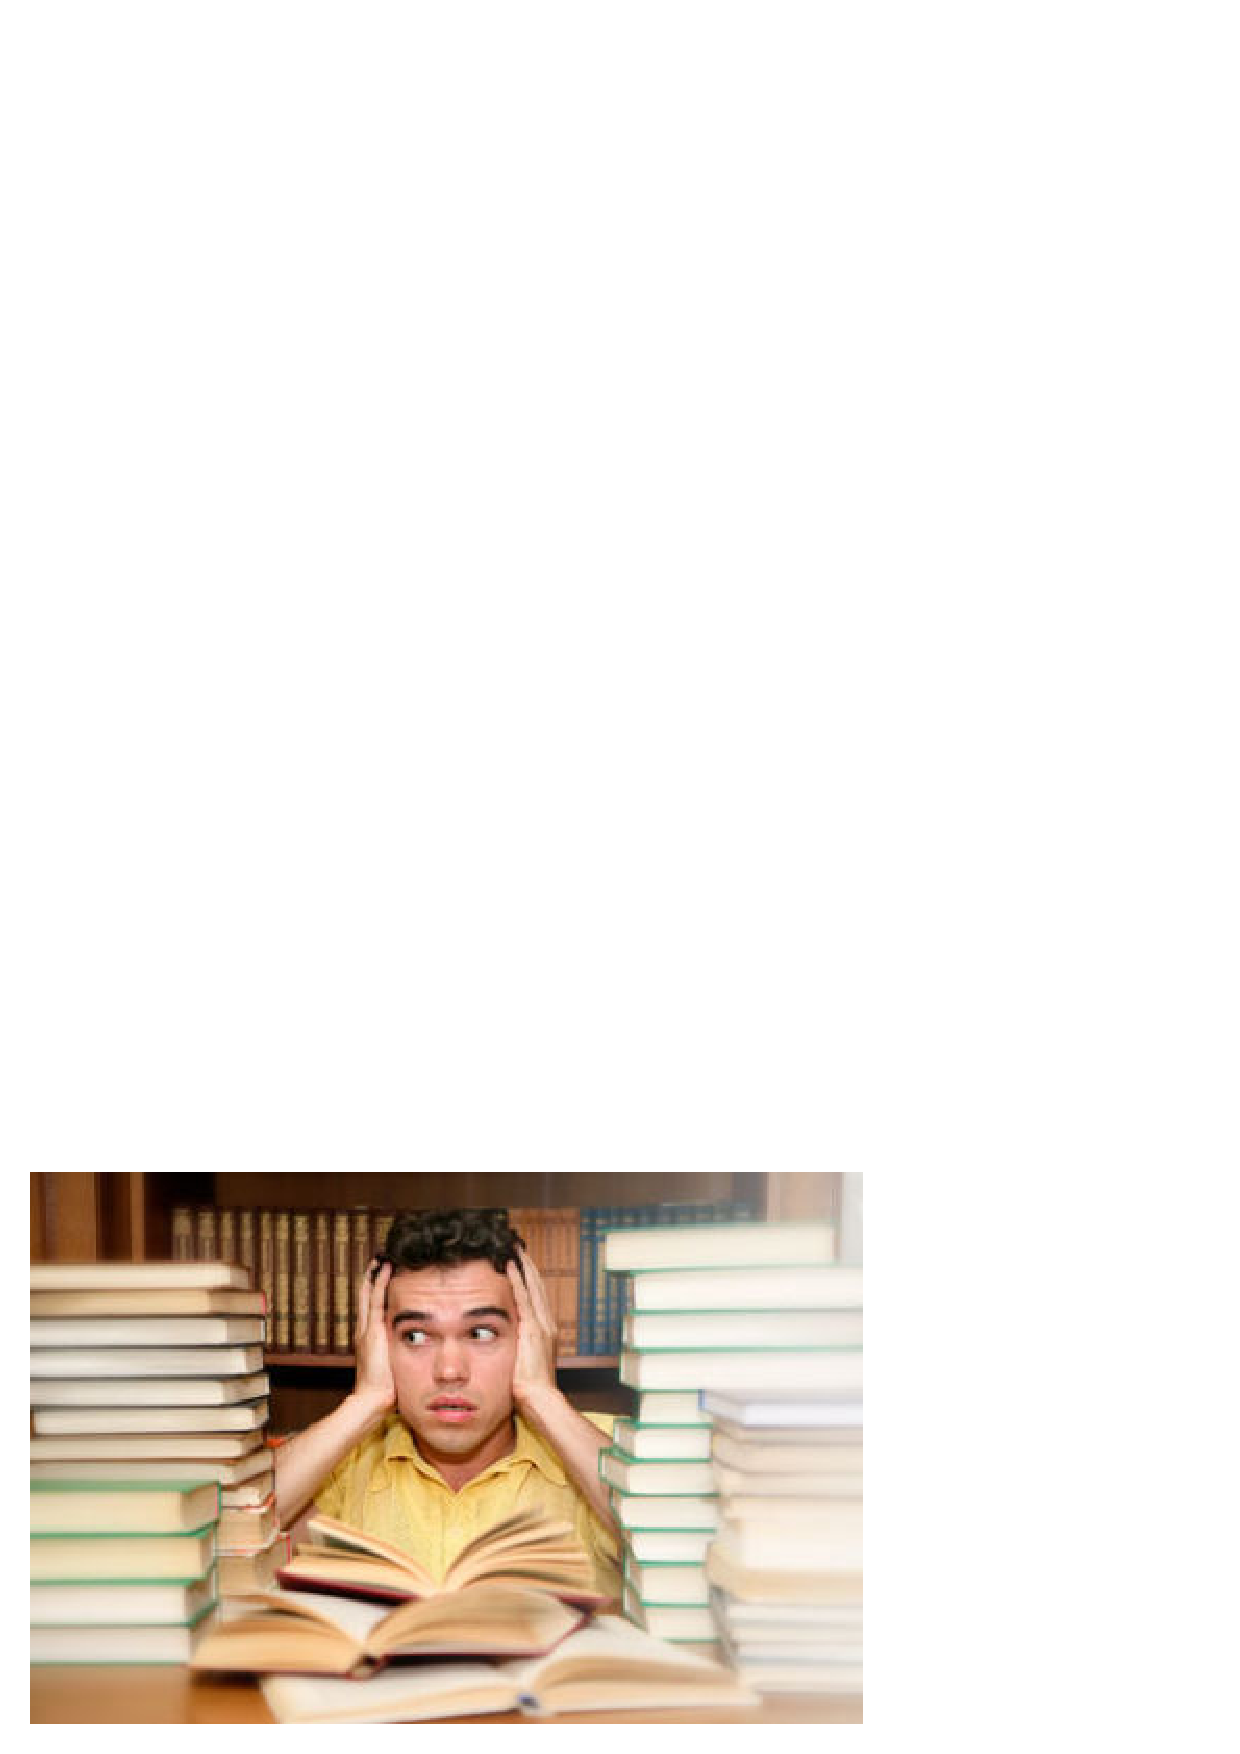
\includegraphics[width=0.9\columnwidth]{studying.pdf}
     \end{minipage}
     \hfill
     \begin{minipage}{0.32\textwidth}
         \centering
         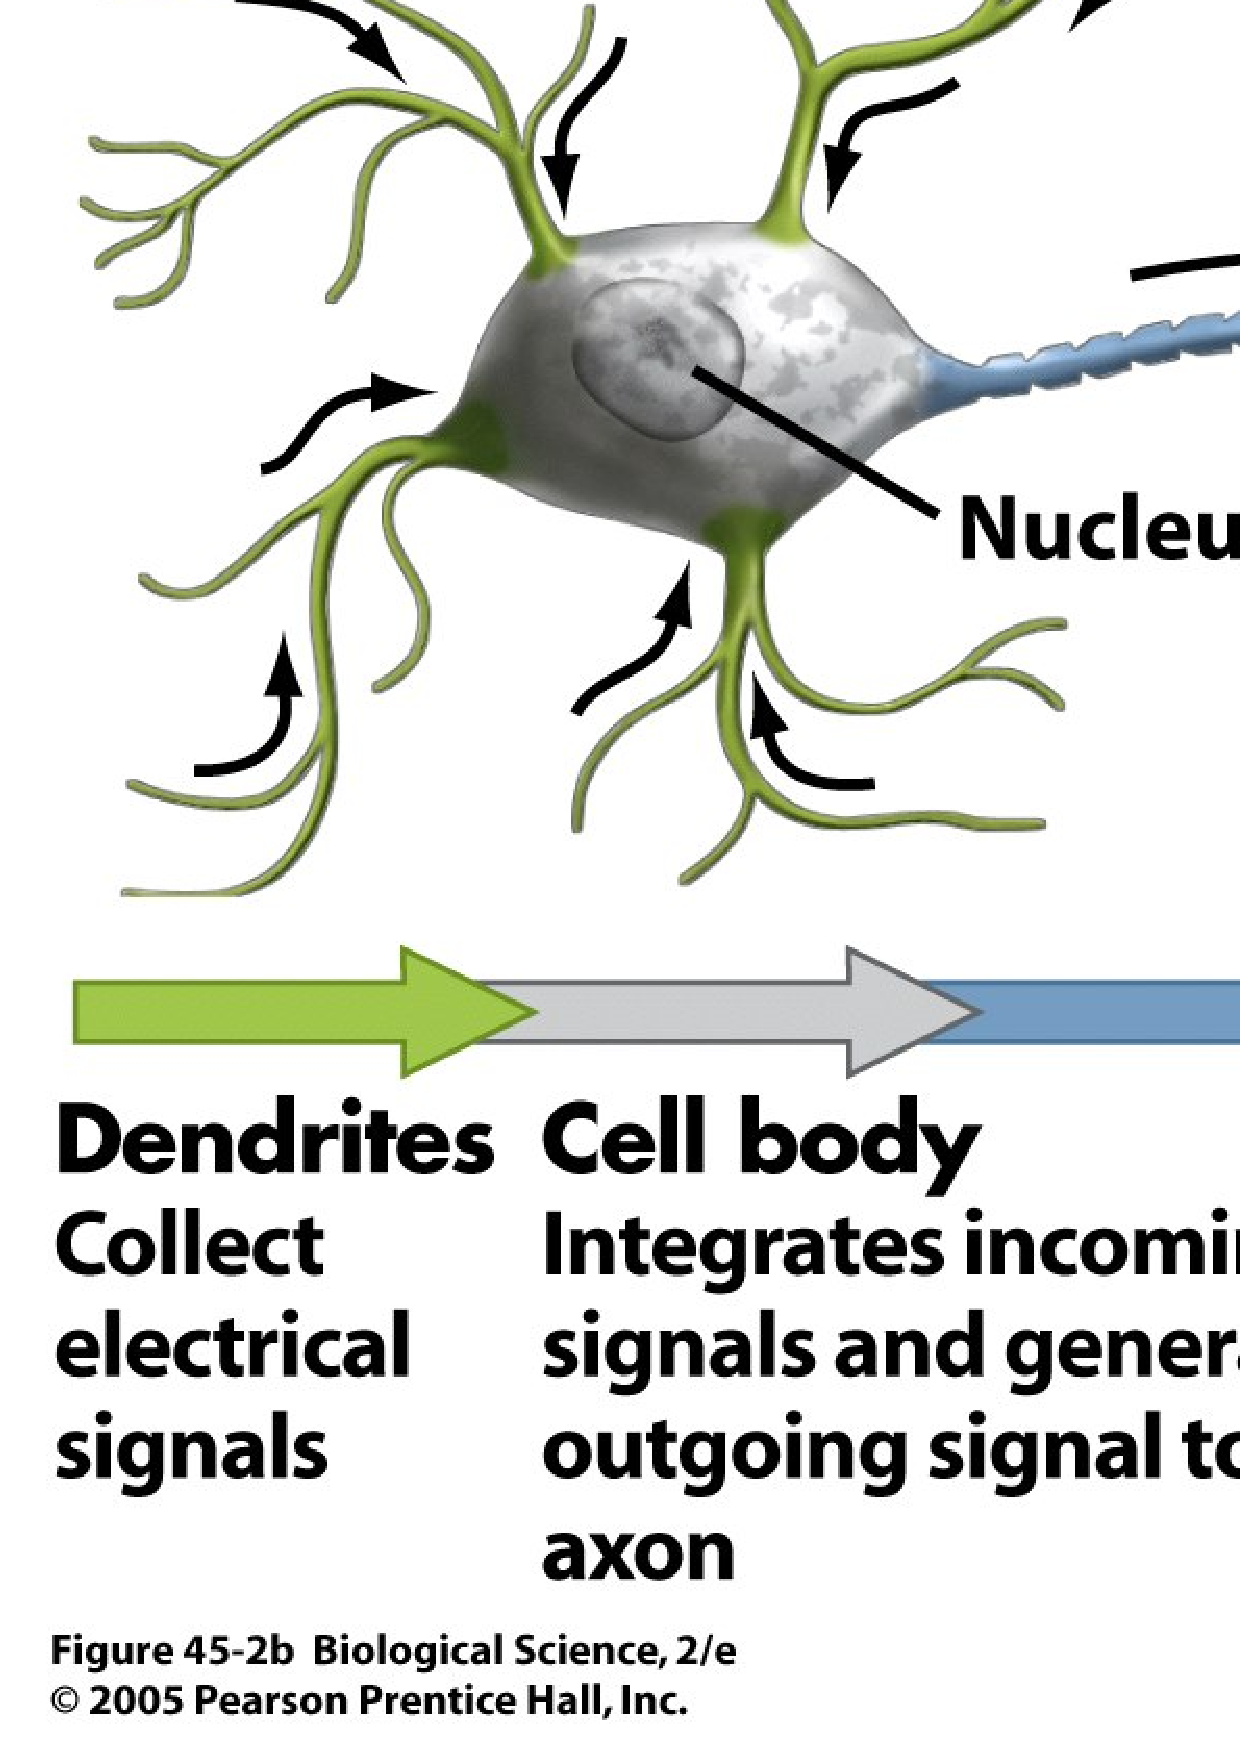
\includegraphics[width=0.9\columnwidth]{neuron.pdf}
     \end{minipage}
     \hfill
     \begin{minipage}{0.32\textwidth}
         \centering
         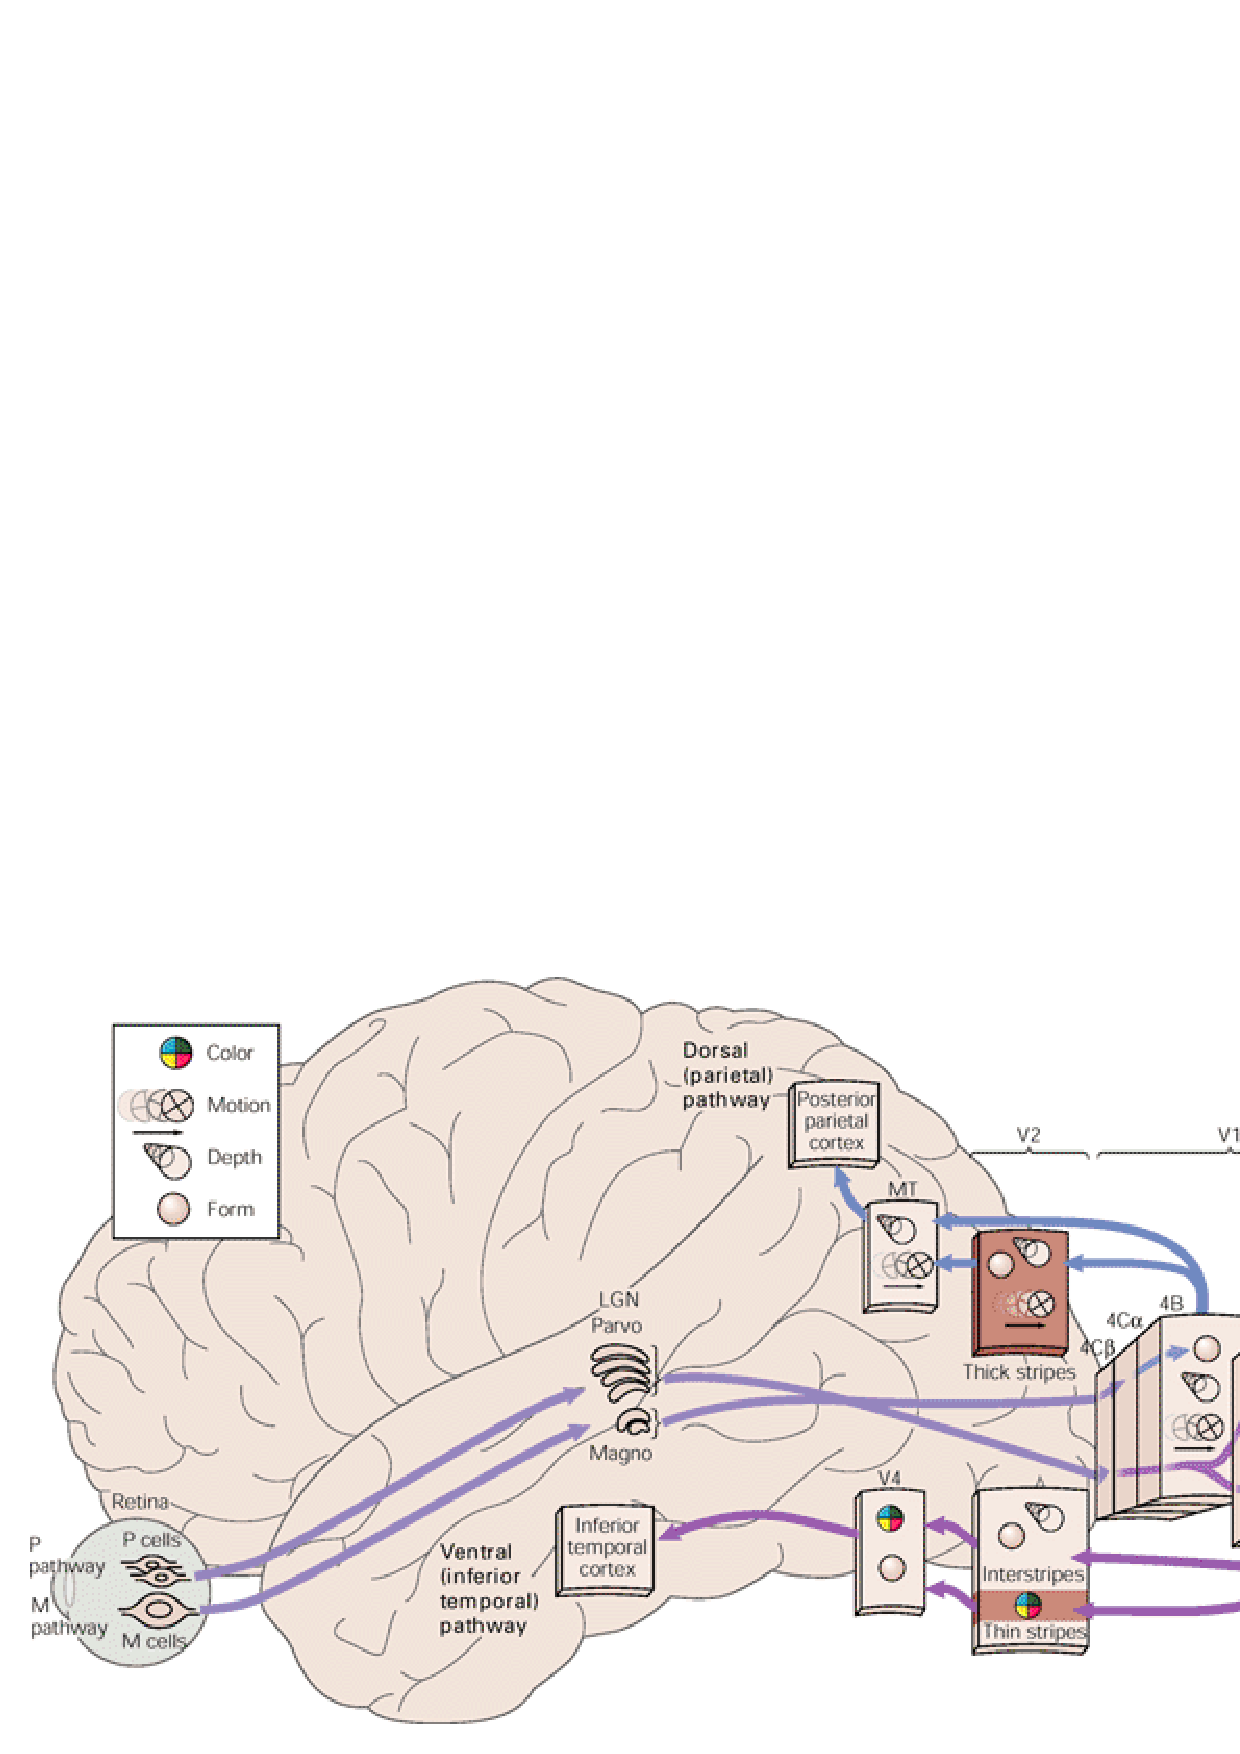
\includegraphics[width=0.9\columnwidth]{visual_pathway.pdf}
         \\
         \raggedleft {\tiny (Van Essen\&Gallant, 1994)}
     \end{minipage}

     \begin{minipage}{0.32\textwidth}
         \centering
         \small
         \textit{Learn} massive data
     \end{minipage}
     \hfill
     \begin{minipage}{0.32\textwidth}
         \centering
         \small
         \textit{simple functions}
     \end{minipage}
     \hfill
     \begin{minipage}{0.32\textwidth}
         \centering
         \small
         \textit{Multi-layered} 
     \end{minipage}

     \vspace{3mm}
    \centering
    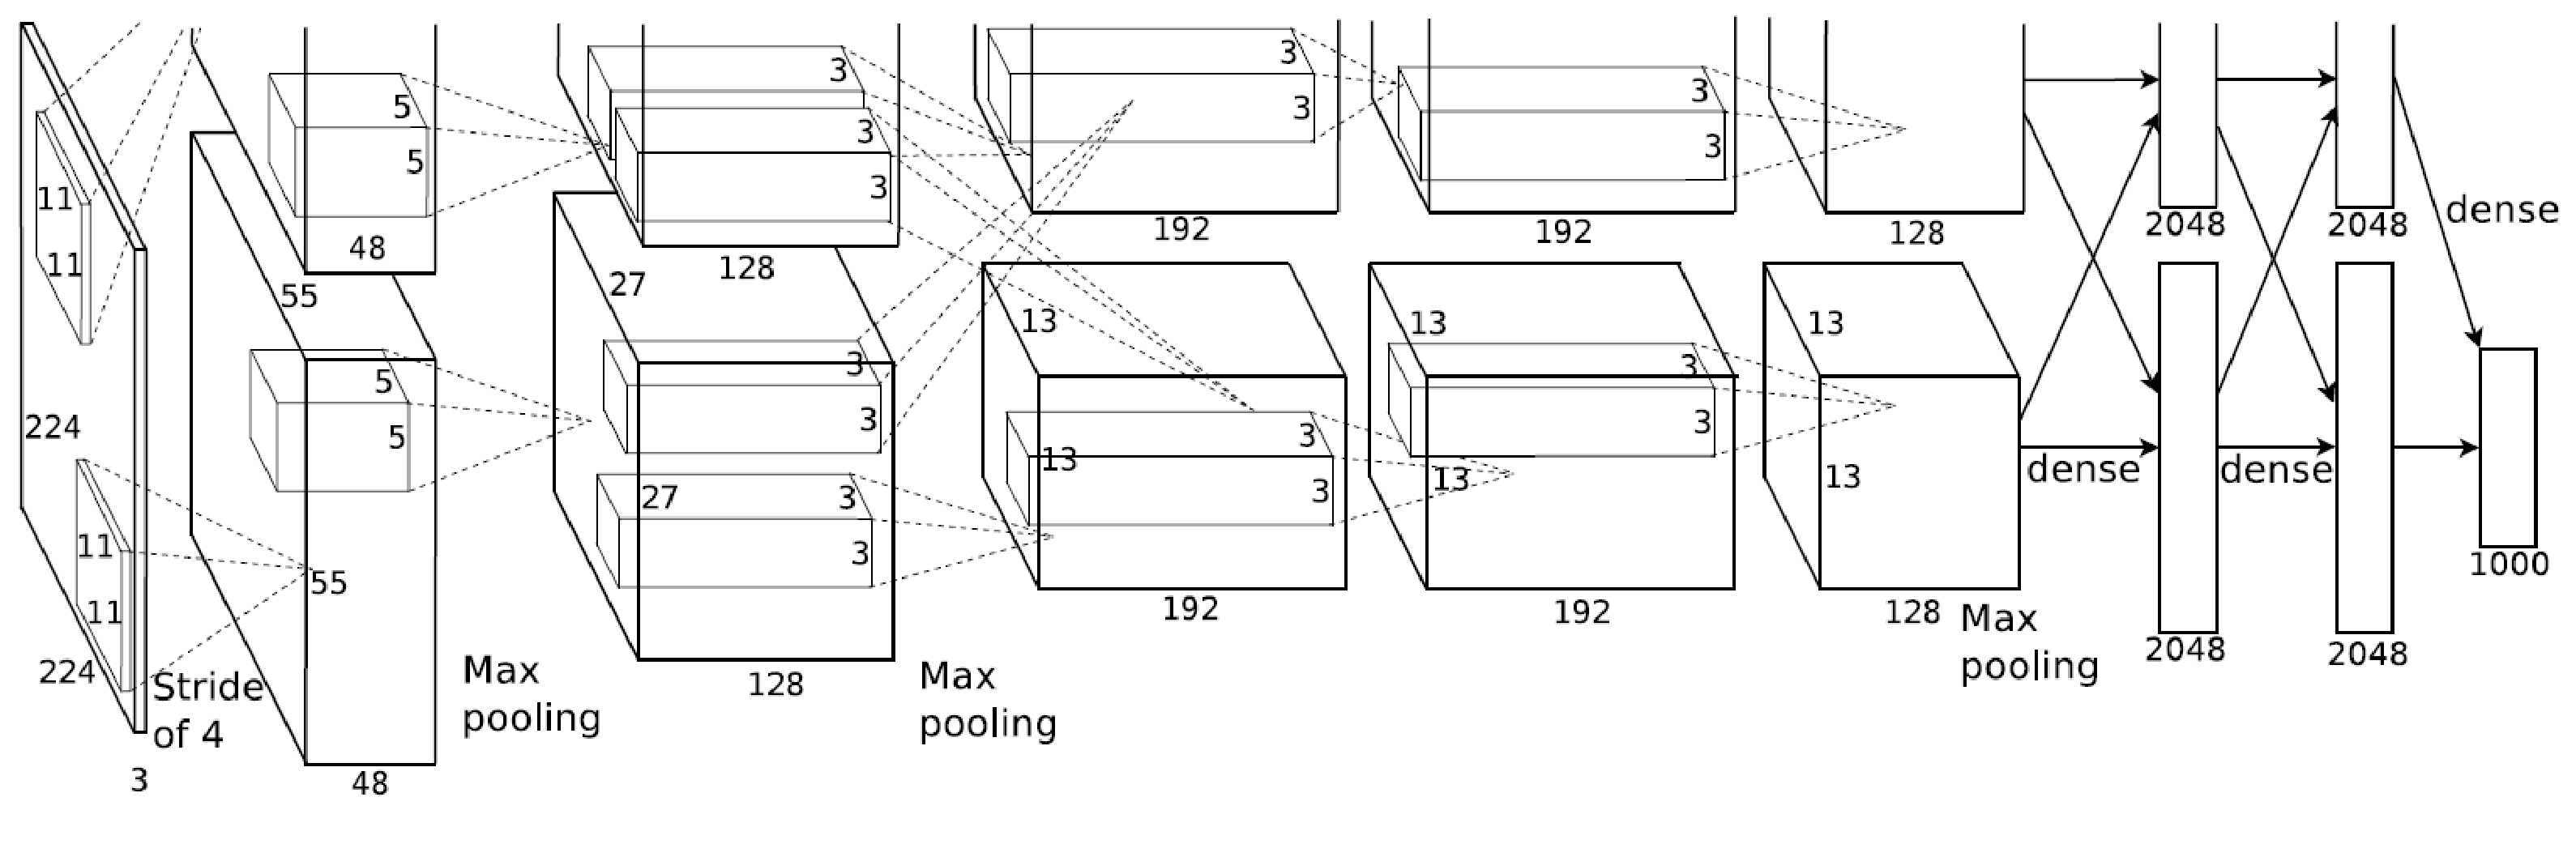
\includegraphics[width=0.8\textwidth]{alex_imagenet}
    \\
    \raggedleft {\scriptsize (Krizhevsky et al., 2012)}

    \vfill

\end{frame}

\begin{frame}{Conventional Machine Learning}
    \raggedright
    \begin{enumerate}
        \item Feature engineering $\leftarrow$ {\bf \emph{not learned!}}
        \item \tred{Learning}
        \item \tblue{Inference}
    \end{enumerate}

    \vspace{-24mm}
    \begin{center}
    \includegraphics[width=0.8\textwidth]{pipeline1.pdf}
    \end{center}

\end{frame}

\begin{frame}{Deep Learning (1)}
    \raggedright
    \begin{enumerate}
        \item Jointly \tred{learn} \emph{everything}
        \item \tblue{Inference}
    \end{enumerate}

    \vspace{-24mm}
    \begin{center}
    \includegraphics[width=0.8\textwidth]{pipeline3.pdf}
    \end{center}

\end{frame}

\begin{frame}{Deep Learning (2): Learning Representation}
    \raggedright
    \begin{enumerate}
    \itemsep 0em
        \item[1a.] Feature engineering
        \item[1b.] Feature/Representation \tred{learning}
        \item[2.] \tred{Learning}
        \item[3.] \tblue{Inference}
    \end{enumerate}

    \vspace{-28mm}
    \begin{center}
    \includegraphics[width=0.8\textwidth]{pipeline2.pdf}
    \end{center}

\end{frame}

\subsection{Deep Learning: Born Again}

\begin{frame}{Deep Learning: Old Technology}

\begin{enumerate}
\item[1958] Rosenblatt proposed perceptrons 
\item[1982] Hopfield network, SOM {\scriptsize (Kohonen, 1982)}, Neural PCA {\scriptsize (Oja, 1982)}
\item[1985] Boltzmann machines {\scriptsize (Ackley et al., 1985)}
\item[1986] Multilayer perceptrons and backpropagation {\scriptsize (Rumelhart et al., 1986)}
\item[1988] RBF networks {\scriptsize (Broomhead\&Lowe, 1988)}
\item[1989] Autoencoders {\scriptsize (Baldi\&Hornik, 1989)}, Convolutional network {\scriptsize (LeCun, 1989)}
\item[1992] Sigmoid belief network {\scriptsize (Neal, 1992)}
\end{enumerate}

\end{frame}

\begin{frame}

\centering
\includegraphics[width=0.80\textwidth]{bet-by-2000.jpg}

\end{frame}

\begin{frame}

\centering
\includegraphics[width=0.75\textwidth]{mit_breakthrough_deepl.png}

{\small
\begin{itemize}
\itemsep 0em
\item  Object Detection {\scriptsize (Krizhevsky et al., 2012; Ciresan et al., 2012; Goodfellow et al., 2013)} 
\item Speech Recognition {\scriptsize (Hinton et al., 2012; Dahl et al., 2012; Deng
        et al., 2013)} 
\item Natural language processing {\scriptsize (Socher et al., 2011; Mikolov et al., 2010)} 
\item Transfer learning {\scriptsize (Mesnil et al., 2012)}
\end{itemize}
}

\end{frame}

\subsection{Challenges}

\begin{frame}{Challenges in Machine Learning}
    \centering
    \includegraphics[width=0.55\textwidth]{machinelearning.pdf}

    \vspace{4mm}
    \raggedright
    \begin{enumerate}
        \item \tred{Learning} is \emph{not} trivial 
        \item \tred{Learning} and \tblue{inference} are \emph{not} separate
    \end{enumerate}
\end{frame}

\begin{frame}{Learning Difficulties}

    \centering
    \begin{minipage}{0.48\textwidth}
    \centering
    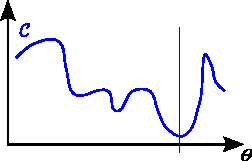
\includegraphics[width=\columnwidth]{cost_true.pdf}
    \end{minipage}
    \hfill
    \begin{minipage}{0.48\textwidth}
    \centering
    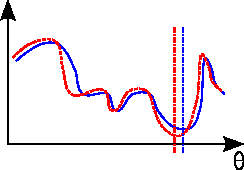
\includegraphics[width=\columnwidth]{cost_both.pdf}
    \end{minipage}

    \vspace{2mm}
    \begin{itemize}
    \item True cost $\color{blue}{\CC}$ is \emph{not} available: Only empirical cost $\color{red}\tilde{\CC}$ available
    \item Often, non-convex optimization with many local/apparent minima
    \item Impractical to compute either $\color{blue}\CC$ or $\color{red}\tilde{\CC}$, as $\left| D \right|\to\infty$
    \end{itemize}

\end{frame}

\begin{frame}{Vicious Cycle or Virtuous Cycle?}

    %\begin{minipage}{0.48\textwidth}
        \centering
        \includegraphics[width=0.5\textwidth]{vicious_cycle.pdf}
    %\end{minipage}
    %\hfill
    %\begin{minipage}{0.48\textwidth}
    %    \tred{\emph{Learning}} which changes $\TT$ requires
    %    \tblue{\emph{inferences}} based on $\TT$. 
    %\end{minipage}

    \vfill
    \raggedright
    Example: MLE for feedforward neural networks
    \begin{align*}
        {\color{red} \min_{\TT} \CC(\TT)} \approx 
        {\color{red} \min_{\TT} \tilde{\CC}(\TT)} =
        {\color{red} \min_{\TT} -\frac{1}{N}\sum_{\left(\vx,t\right) \in D}
        \log {\color{blue}p(y=t \mid \vx, \TT)}}
    \end{align*}

\end{frame}

\begin{frame}{What gets worse with \emph{deep} learning?}
    \begin{itemize}
        \item \tred{Learning}
            \begin{itemize}
                \item No access to $\CC$, but only to $\tilde{\CC}$
                \item Highly entangled inference and learning
                \item \textbf{High-dimensional}
                \item \textbf{Non-convex with a lot of local (apparent) minima}
                \item \textbf{Intractable to compute even $\tilde{\CC}$}, because $\left| D \right| \to \infty$
            \end{itemize}
    \end{itemize}

    \begin{itemize}
        \item \tblue{Inference}
            \begin{itemize}
                \item \textbf{No analytical expression}, often
                \item \textbf{Intractable to compute}, often
                \item Difficult to analyze and understand
            \end{itemize}
    \end{itemize}
\end{frame}

\section{Deep, Unsupervised Neural Networks}

\begin{frame}{}
    \begin{center}
    Deep, Unsupervised Neural Networks \\
    Boltzmann Machines and Autoencoders
\end{center}

{\scriptsize
\begin{enumerate}
    \item[\textbf{I}] Enhanced
Gradient for Training Restricted Boltzmann Machines

    \item[\textbf{II}] Enhanced Gradient and Adaptive
        Learning Rate for Training Restricted Boltzmann
        Machines

\item[\textbf{III}] 
Parallel Tempering is Efficient for Learning Restricted Boltzmann Machines

\item[\textbf{VII}] A Two-Stage Pretraining Algorithm for
Deep Boltzmann Machines

\item[\textbf{VIII}] Simple Sparsification Improves Sparse Denoising Autoencoders
in Denoising Highly Corrupted Images
\end{enumerate}
}

\end{frame}

\subsection{Restricted Boltzmann Machines}

\begin{frame}{Boltzmann Machines}

    \begin{minipage}{0.33\textwidth}
        \begin{minipage}{\columnwidth}
            \centering
            \includegraphics[width=0.99\columnwidth]{boltzmann.pdf}
        \end{minipage}
        
        \vspace{3mm}

        \begin{minipage}{\columnwidth}
            \small 
            Popular variants:
            \begin{itemize}
                \item If $\mV=\mzero$ and $\mU=\mzero$, restricted Boltzmann
                    machine (RBM)
                \item If $\mU=\mzero$ and layered $\vh$, deep Boltzmann
                    machine (DBM)
            \end{itemize} 
        \end{minipage}
    \end{minipage}
    \hfill
    \begin{minipage}{0.65\textwidth}
        \small
        \begin{enumerate}
            \item Negative energy over $\vx$ and $\vh$:
                \begin{align*}
                -E(\vx, \vh &\mid \TT) = \vb^\top \vx +
                \vc^\top \vh + \\
                &
                \vx^\top \mW \vh + \frac{1}{2} \vx^\top \mU \vx +
                \frac{1}{2} \vh^\top \mV \vh
            \end{align*}
            \item Probability over $\vx$ and
                $\vh$:
                \begin{align*}
                p(\vx, \vh \mid \TT) = \frac{1}{Z(\TT)} \exp \left\{
                -E\left(\vx , \vh \mid \TT\right)
                \right\}
            \end{align*}
            \item Learn $p(\vx)$ by maximizing
                \begin{align*}
                    \LL(\TT) =& \E_{\vx \in D} \left[ \log
                    \frac{1}{Z(\TT)} \sum_{\vh}
                    e^{-E\left( \vx, \vh \mid \TT\right)}
    \right]
            \end{align*}
            with stochastic gradient descent
        \end{enumerate}
    \end{minipage}
\end{frame}

\begin{frame}{Learning: Observations}
    \begin{minipage}{0.59\textwidth}
        \begin{center}
            \includegraphics[width=\textwidth]{transf.pdf}
        \end{center}
    \end{minipage}
    \hfill
    \begin{minipage}{0.4\textwidth}
        \small 
        \begin{itemize}
            \item Invariant to bit-flipping transformation
            \item $2^{p+q}$ descent directions 
            \item leading to (potentially all) different solutions
            \item Which direction?
            \item How to tractably decide?
        \end{itemize}
    \end{minipage}
\end{frame}

\begin{frame}{Learning: Enhanced Gradient}
    \begin{minipage}{0.35\textwidth}
        \begin{minipage}{\columnwidth}
            \begin{center}
                \includegraphics[width=0.6\textwidth]{enhgrad.png}
            \end{center}
        \end{minipage}

        \vspace{2mm}

        \begin{minipage}{\columnwidth}
            \scriptsize
            \begin{center}
                Covariance of Weight Updates
            \end{center}
        \end{minipage}
        \\
        \begin{minipage}{0.49\columnwidth}
            \begin{minipage}{\columnwidth}
                \begin{center}
                    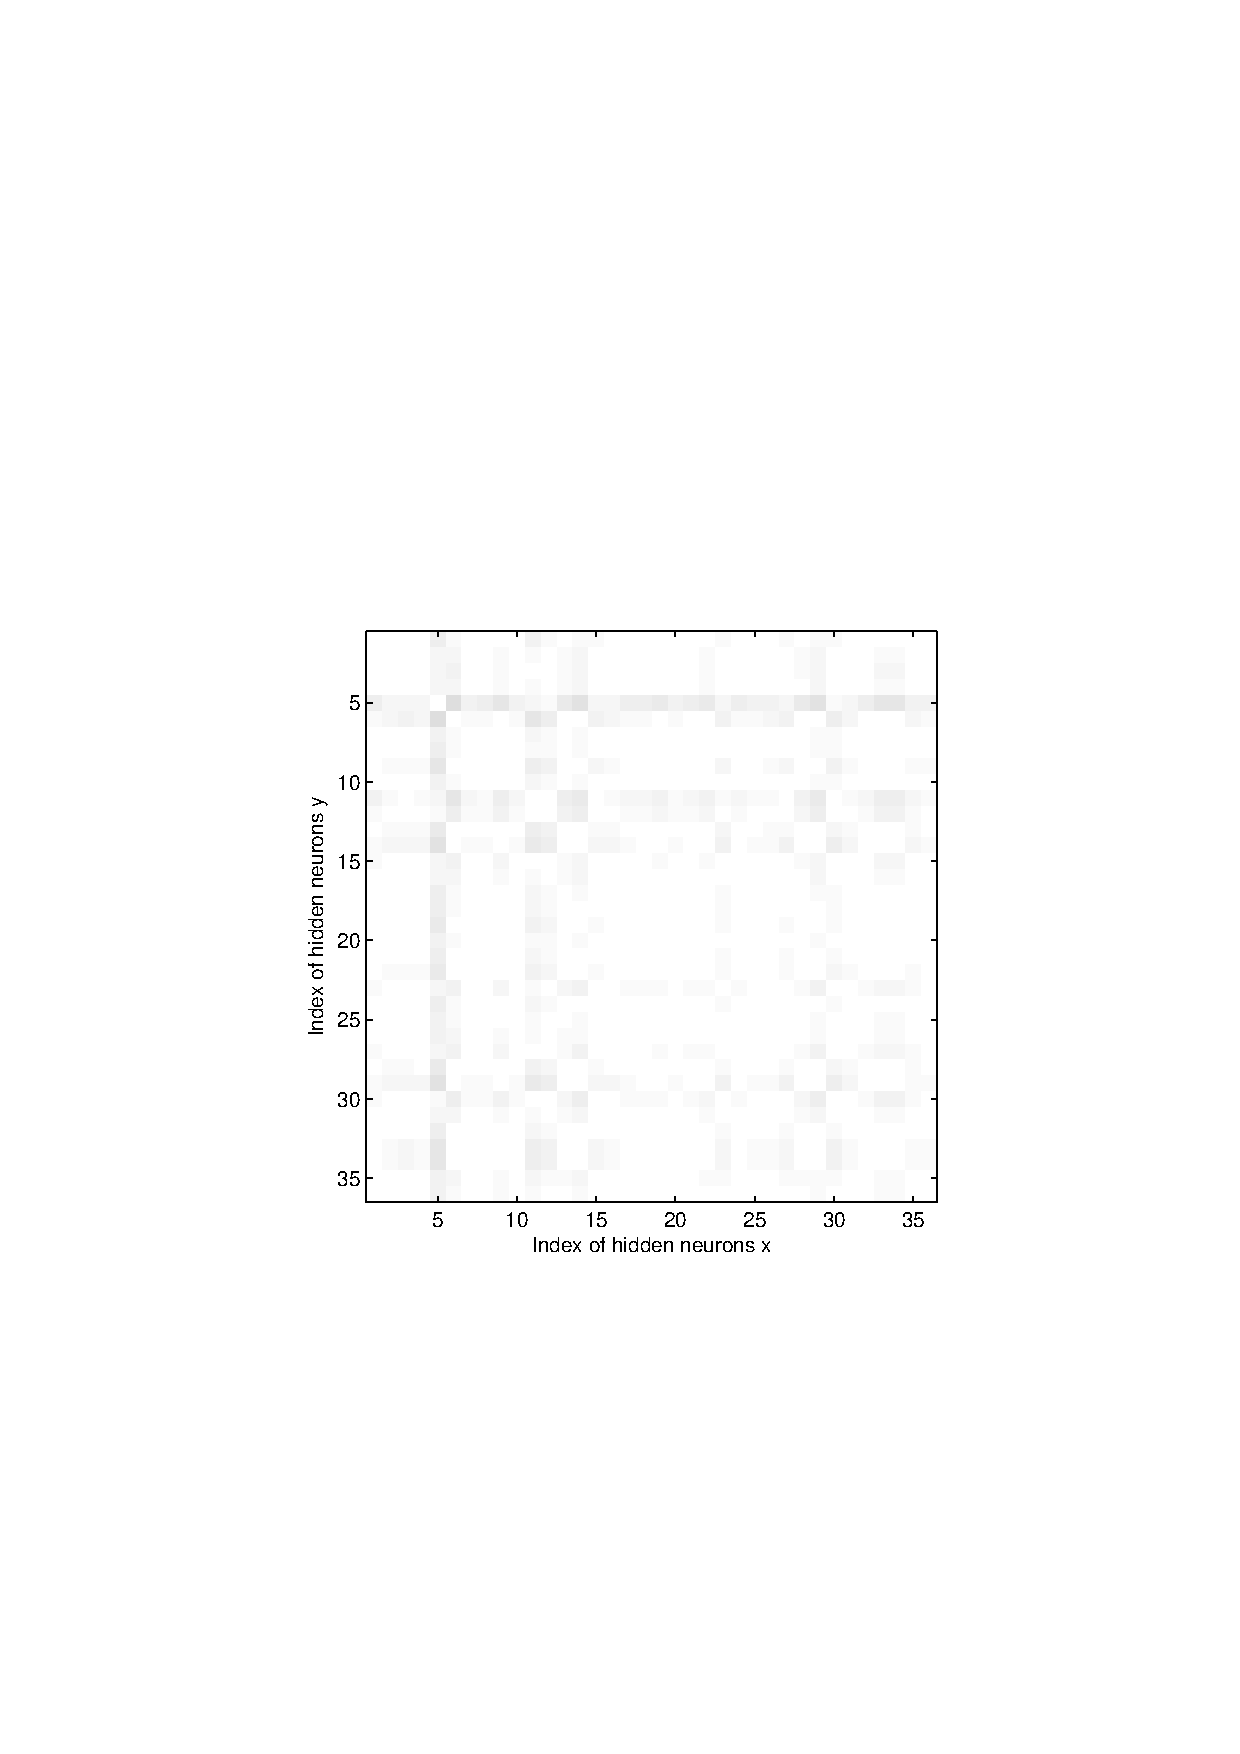
\includegraphics[width=\columnwidth,trim=93 35 75 20,clip=true]{norm_grad_cov.pdf}
                \end{center}
            \end{minipage}
            \begin{minipage}{\columnwidth}
                \begin{center}
                    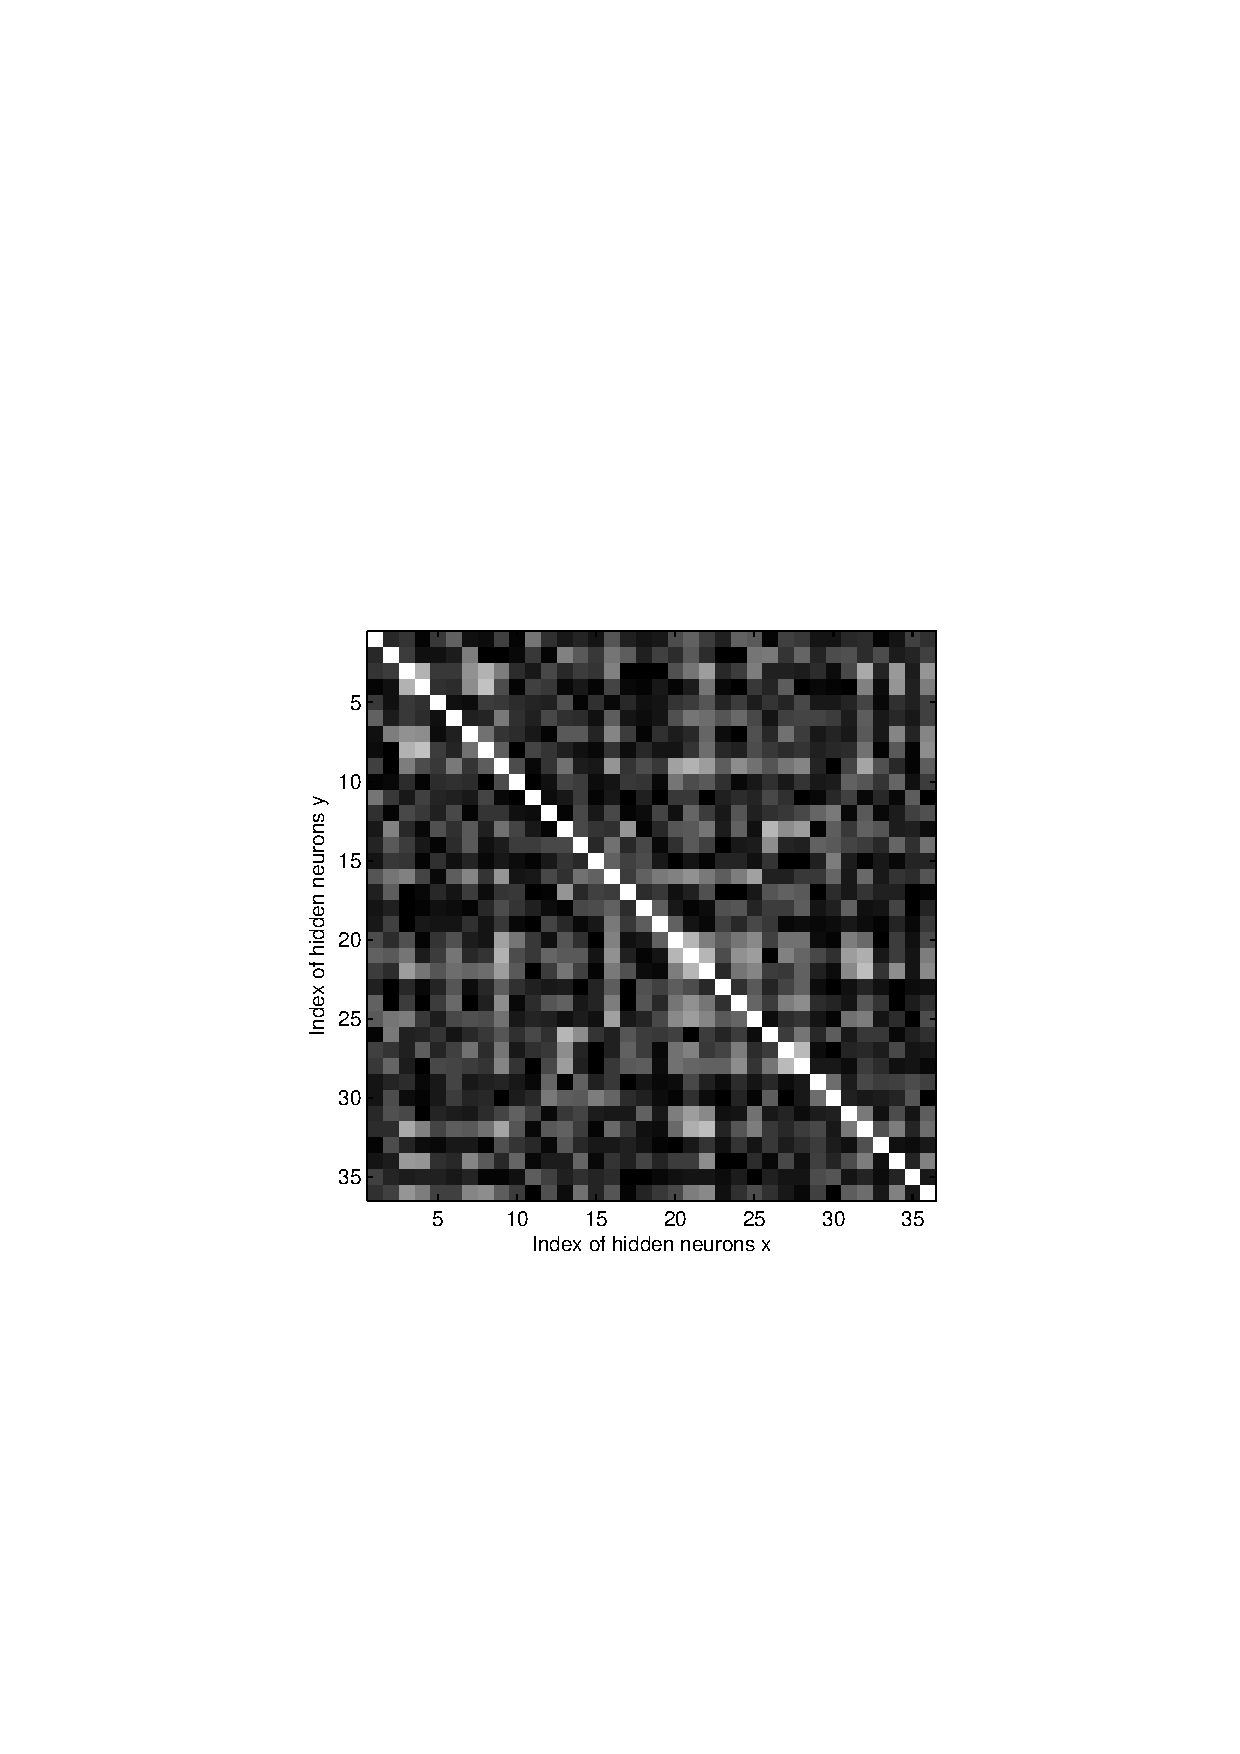
\includegraphics[width=\columnwidth,trim=93 35 75 20,clip=true]{enh_grad_cov.pdf}
                \end{center}
            \end{minipage}
        \end{minipage}
        \hfill
        \begin{minipage}{0.49\columnwidth}
            \begin{minipage}{\columnwidth}
                \begin{center}
                    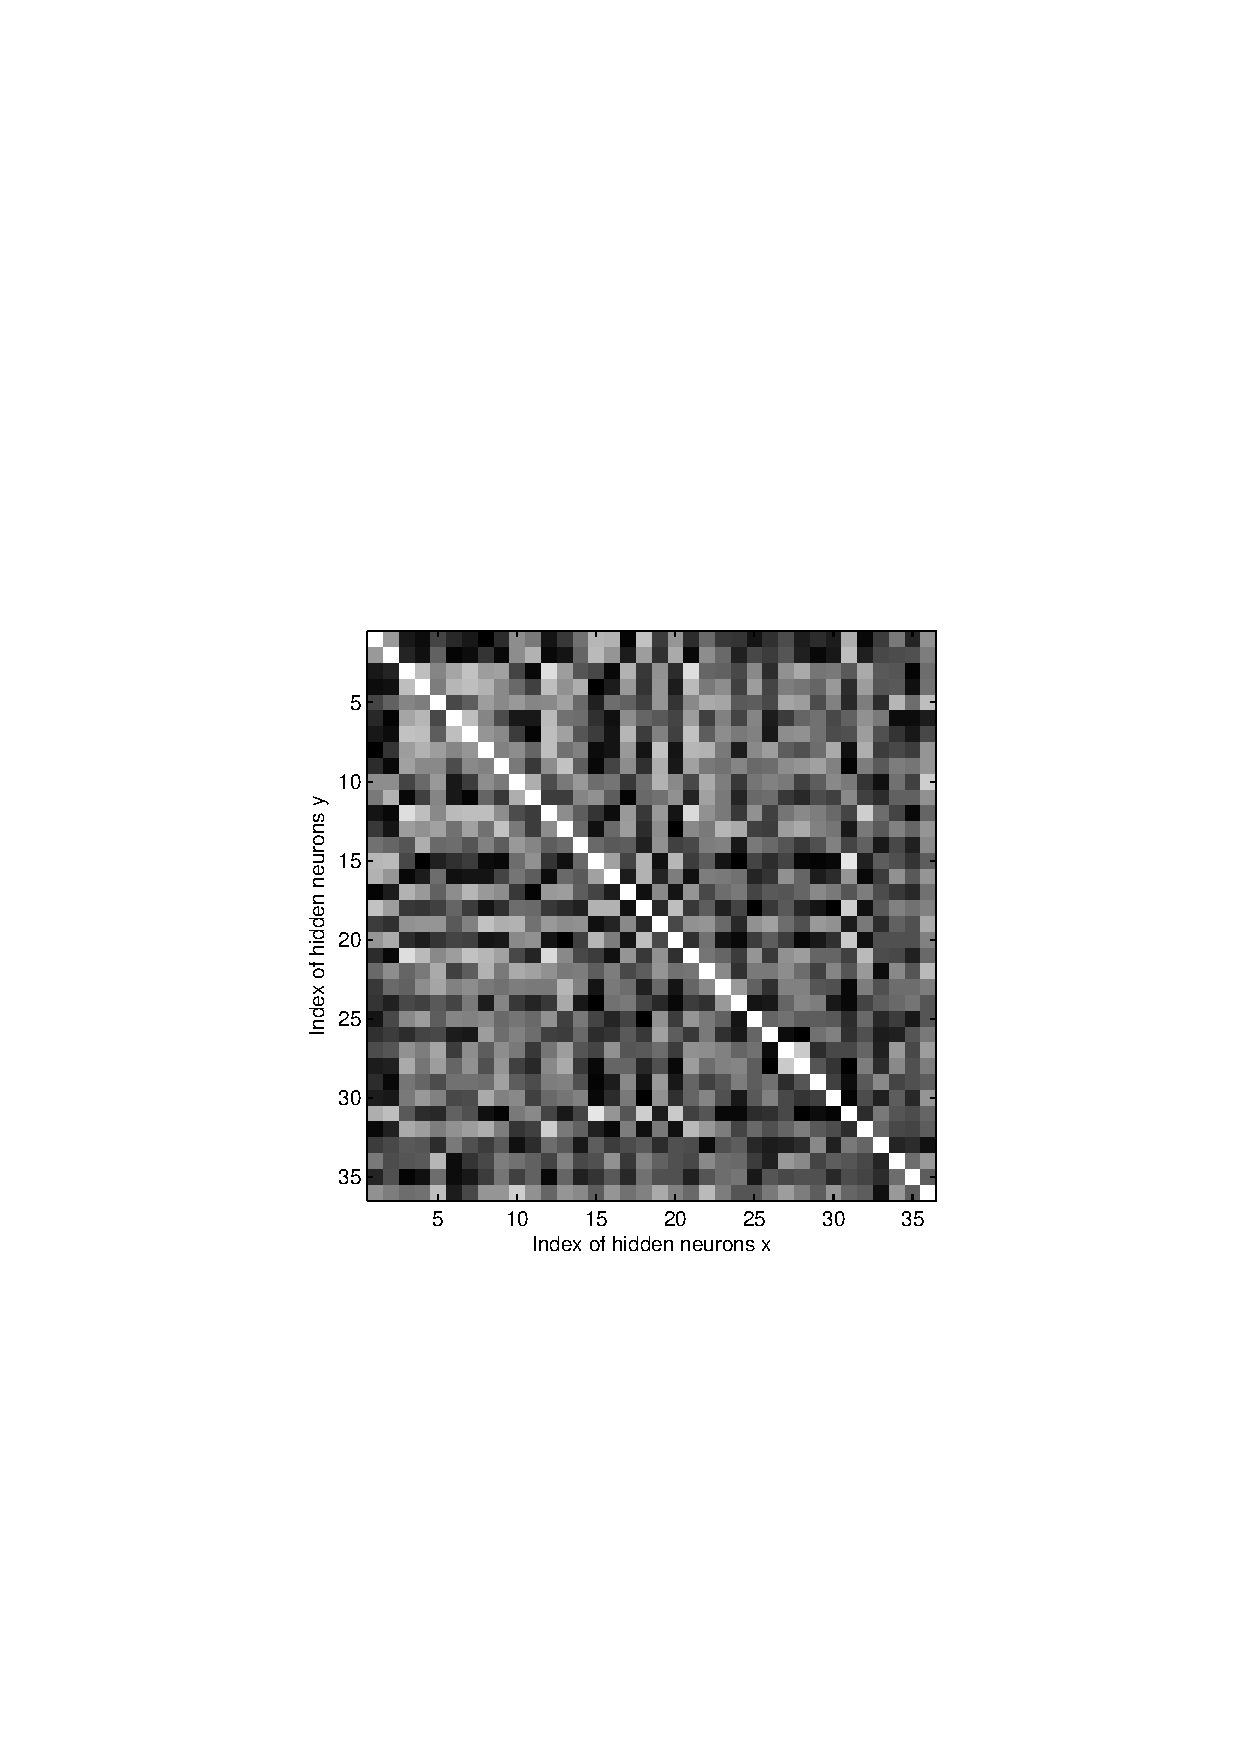
\includegraphics[width=\columnwidth,trim=93 35 75 20,clip=true]{norm_grad_cov_later.pdf}
                \end{center}
            \end{minipage}
            \begin{minipage}{\columnwidth}
                \begin{center}
                    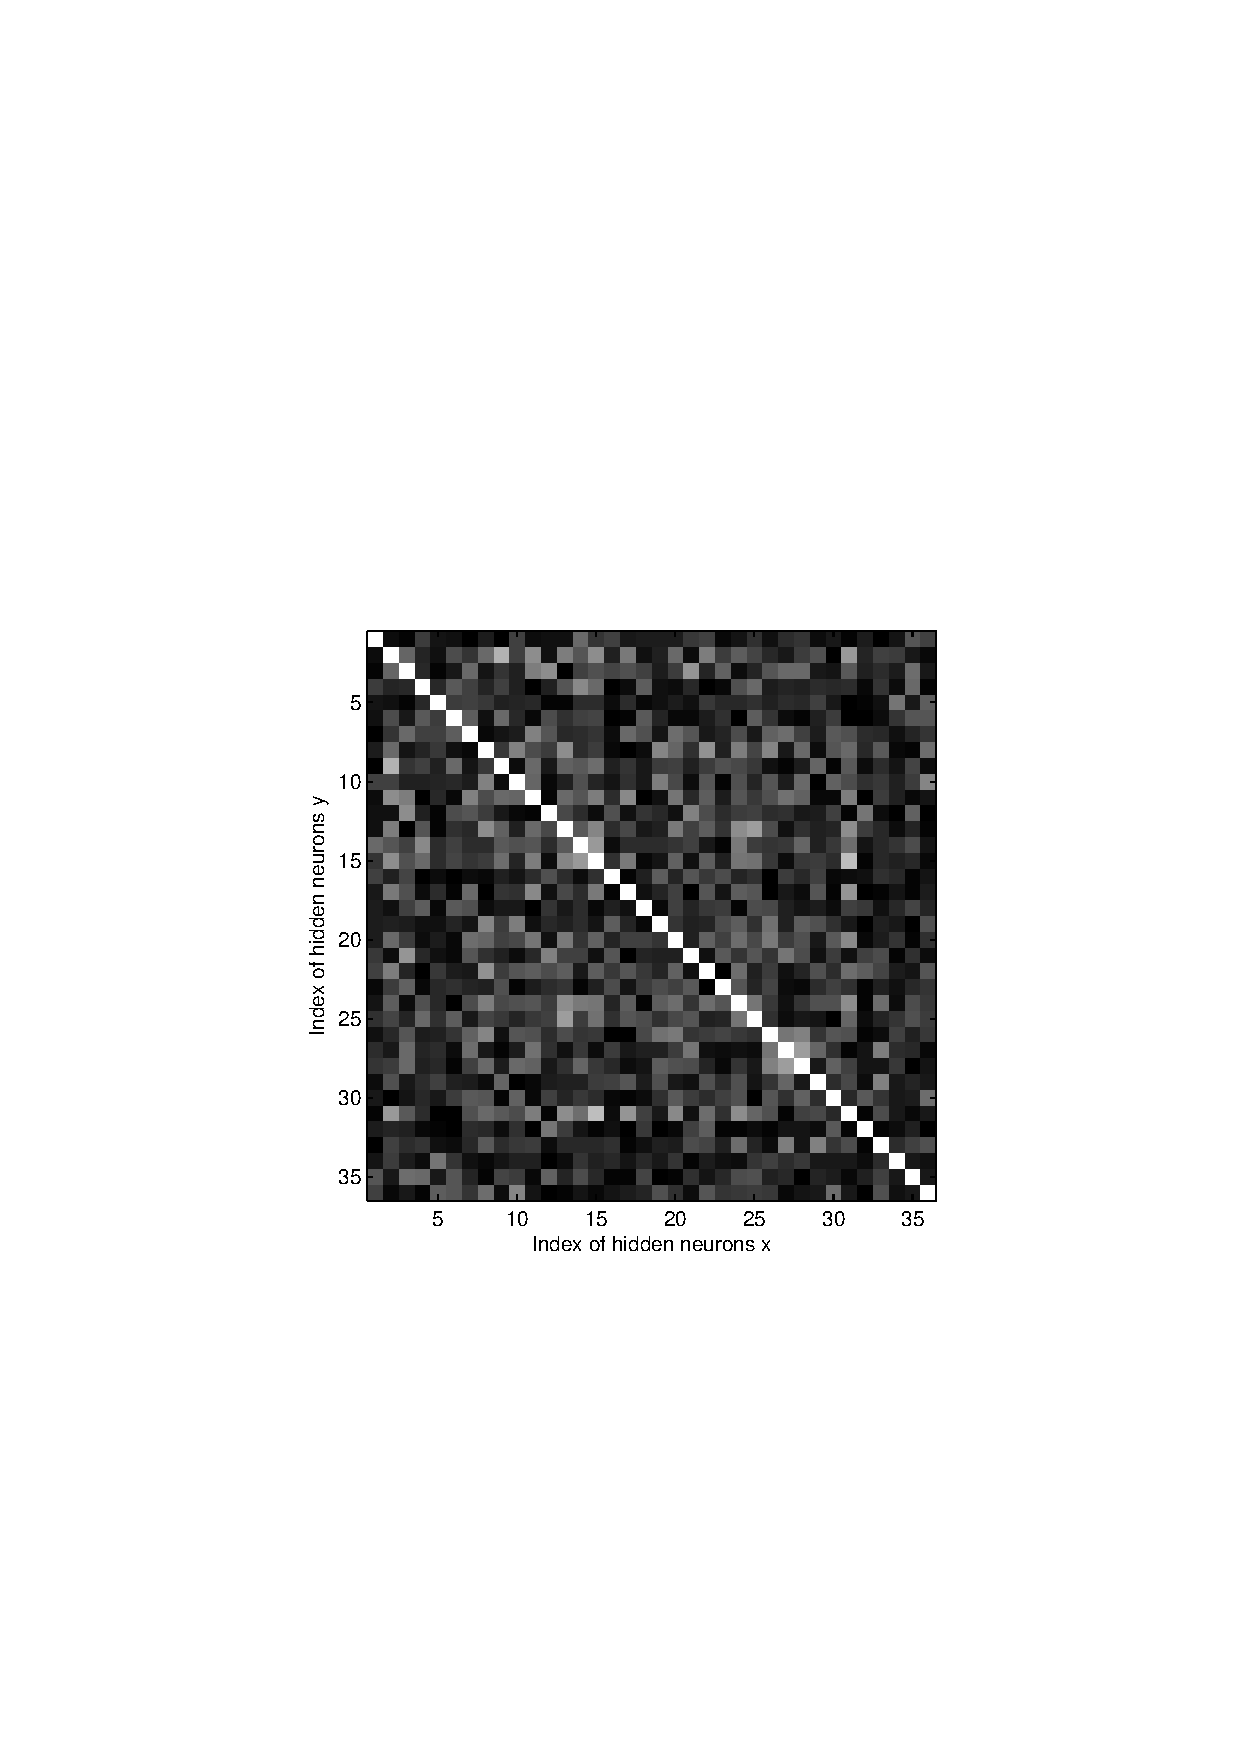
\includegraphics[width=\columnwidth,trim=93 35 75 20,clip=true]{enh_grad_cov_later.pdf}
                \end{center}
            \end{minipage}
        \end{minipage}
        \\
        \begin{minipage}{0.49\columnwidth}
            \scriptsize
            \begin{center}
                Conventional
            \end{center}
        \end{minipage}
        \hfill
        \begin{minipage}{0.49\columnwidth}
            \scriptsize
            \begin{center}
                Enhanced
            \end{center}
        \end{minipage}
    \end{minipage}
    \hfill
    \begin{minipage}{0.64\textwidth}
        \small 
        \begin{itemize}
            \item Importance/weight of each direction $\nabla_{\vf} \LL$
                \begin{align*}
                    \prod_{k=1}^{n_v+n_h} \qexp{x_k}_\tdf^{f_k}
                    \left( 1 - \qexp{x_k}_\tdf
                    \right)^{1-f_k} 
                \end{align*}

            \item Weighted sum of all possible updates 
            \begin{align*}
                \enhnabla w_{ij} &= \cov_\td\left(x_i, h_j\right)
                - \cov_\tf\left(x_i, h_j\right)
                \\
                \enhnabla b_i &= \left<x_i\right>_\td - \left<x_i\right>_\tf
                - \sum_j \qexp{ h_j }_\tdf
                \enhnabla w_{ij}
                \\
                \enhnabla c_j &= \left<h_j\right>_\td - \left<h_j\right>_\tf
                - \sum_i \qexp{ x_i }_\tdf
                \enhnabla w_{ij}
            \end{align*}
        \end{itemize}
    \end{minipage}
\end{frame}

\begin{frame}{Learning vs. Inference}
\begin{itemize}
    \item Boltzmann machine \tred{learning} requires
    \tblue{inference}.
    \begin{align*}
        {\color{red} \enhnabla w_{ij}} &= {\color{black}\cov_\td\left(x_i,
        h_j\right)}
        - {\color{blue}\cov_\tf\left(x_i, h_j\right)}
    \end{align*}
    \end{itemize}

    \begin{itemize}
        \item \emph{What is the covariance between $x_i$ and $h_j$ with the
    current $\TT$?} 
    \begin{itemize}
        \item NP-Hard problem even in the case of RBMs {\small (Long\&Servedio, 2010)}
        \item Monte Carlo approximation with persistent MCMC
            \[
            {\color{blue}\cov_\tf\left(x_i, h_j\right)}
            \approx
            \left(\frac{1}{N} \sum_{n=1}^N x_i^{(n)}
            h_j^{(n)}\right) - 
            \left( 
            \frac{1}{N} \sum_{n=1}^N x_i^{(n)} 
            \right)
            \left(\frac{1}{N}
            \sum_{n=1}^N h_j^{(n)}
            \right)
            \]
        \item Gibbs sampling
    \end{itemize}
    \end{itemize}
\end{frame}

\begin{frame}{Learning vs. Inference: Vicious Cycle}

    \begin{center}
        \includegraphics[width=0.9\textwidth]{vicious_cycle_bm.pdf}
    \end{center}

    \raggedright
    Failed \tblue{inference} (sampling) breaks
            \tred{learning} 

    \raggedleft
            $\to$ \emph{Good MCMC sampler is
            needed!}

\end{frame}

\begin{frame}{Inference: Better MCMC Sampler}
\begin{minipage}{0.49\textwidth}
\centering
\scriptsize
Gibbs sampling
\end{minipage}
\hfill
\begin{minipage}{0.49\textwidth}
\centering
\scriptsize
Parallel Tempering
\end{minipage}
\\
\begin{minipage}{0.49\textwidth}
\centering
\includegraphics[width=.9\textwidth]{bad_inference_bm.pdf}
\end{minipage}
\hfill
\begin{minipage}{0.49\textwidth}
\centering
\includegraphics[width=.9\textwidth]{parallel_tempering.pdf}
\end{minipage}

\begin{itemize}
\item MCMC with a \emph{local} jump cannot easily escape an isolated mode
\end{itemize}

\begin{minipage}{0.4\textwidth}
\centering
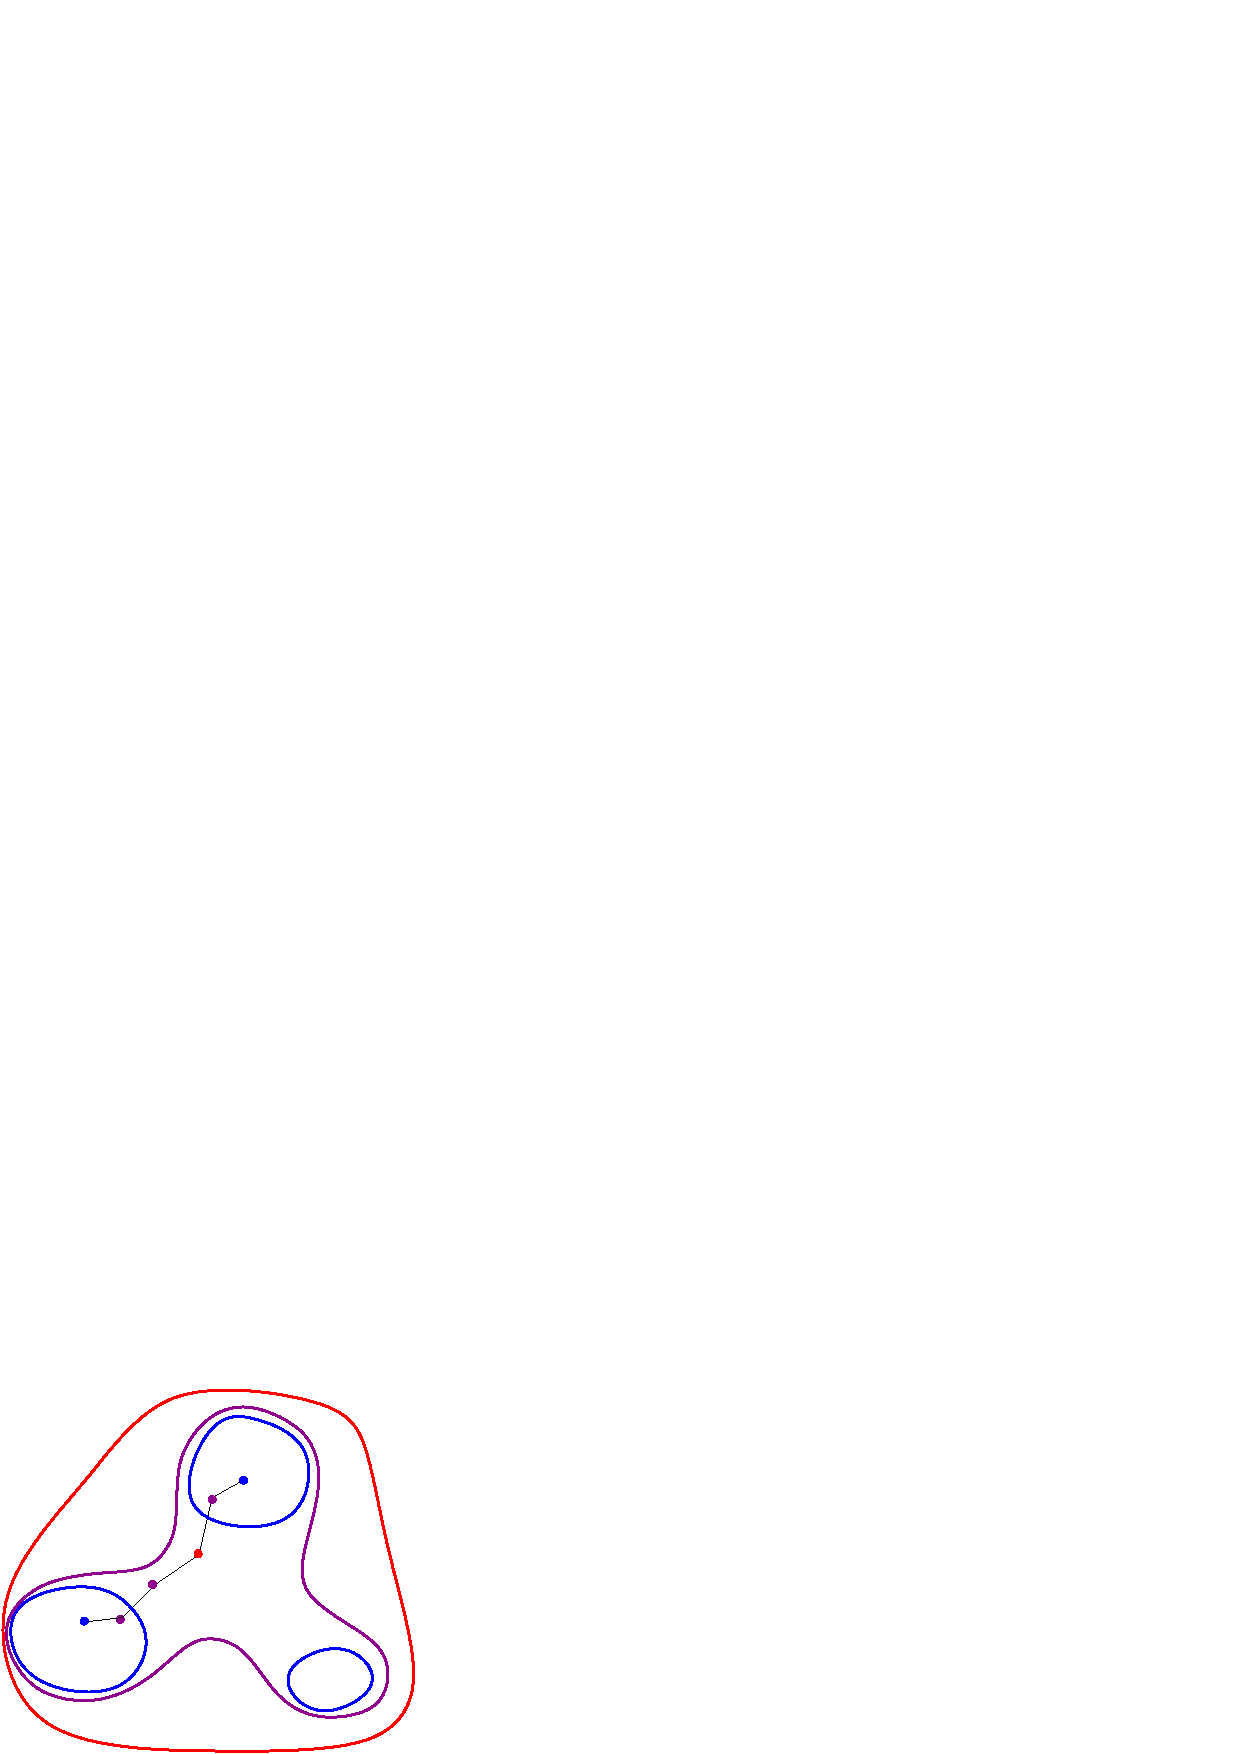
\includegraphics[width=0.8\textwidth]{pt.pdf}
\end{minipage}
\begin{minipage}{0.58\textwidth}
{\bf Parallel Tempering}
\begin{itemize}
\item Parallel chains between $\color{red}P_0$ and $\color{blue}P_{\infty}$
\item Jump via tempered chains
\item Better exploration of the state space
\end{itemize}
\end{minipage}

\end{frame}

\begin{frame}{From an RBM to a \emph{deeper} neural
network..}

\begin{minipage}{0.4\textwidth}
\centering
Deep Belief Network
\\
{ \small
    (Pretrained MLP)
}
\end{minipage}
\begin{minipage}{0.59\textwidth}
\centering
\includegraphics[width=0.9\columnwidth]{mlp_pretrain.pdf}
\end{minipage}

\vfill
\hrulefill
\vfill

\begin{minipage}{0.4\textwidth}
\centering
{\bf
Deep Boltzmann Machine
}
\end{minipage}
\begin{minipage}{0.59\textwidth}
\centering
\includegraphics[width=0.4\columnwidth]{dbm.pdf}
\end{minipage}

 


\end{frame}

\subsection{Deep Boltzmann Machines}

\begin{frame}{Deep Boltzmann Machines}
\begin{minipage}{\textwidth}
\begin{minipage}{0.29\textwidth}
\centering
\includegraphics[width=\columnwidth]{dbm.pdf}
\end{minipage}
\hfill
\begin{minipage}{0.7\textwidth}
\begin{itemize}
\item \emph{Undirected} Hierarchical Model
\item Negative Energy
\end{itemize}

\vspace{-8mm}
\begin{align*}
    -E&(\vx, \vh \mid \TT) = \\
    &\vb^\top \vx +
    \vc_{\qlay{1}}^\top \vh_{\qlay{1}}
    + \vx^\top \mW \vh_{\qlay{1}} \\
    &+\sum_{l=2}^L \left(
    \vc_{\qlay{l}}^\top
    \vh_{\qlay{l}} + \vh_{\qlay{l-1}}^\top \mU_{\qlay{l-1}}
    \vh_{\qlay{l}} \right)
\end{align*}
\end{minipage}
\end{minipage}

\vspace{4mm}
\begin{minipage}{\textwidth}
\begin{itemize}
\item The further away a layer from $\vx$, the more abstract
concept the layer learns
\item Hierarchical representation with both bottom-up and
top-down signals
\end{itemize}
\end{minipage}
\end{frame}

\begin{frame}{Learning: Depressing Observation}

\textbf{Observation}: Lack of Structures in Deeper Hidden Layers

\vspace{4mm}
Which direction does learning move toward? -- matching
\tblue{data} and \tred{model} statistics
\begin{align*}
    \frac{\partial \LL(\TT)}{\partial u^{\qlay{l}}_{ij}} \propto
    \textcolor{blue}{\left< h^{\qlay{l}}_i h^{\qlay{l+1}}_j
    \right>_{p\left(\vh \mid \vv,
    \TT\right)p_D\left(\vv\right) } }
    -
    \textcolor{red}{\left< h^{\qlay{l}}_i h^{\qlay{l+1}}_j
    \right>_{p\left(\vv, \vh \mid \TT\right)}}
\end{align*}

\vspace{4mm}
What happens if \tblue{$p(\vh \mid \vv, \TT)$} does not
have \textit{any} structure?
\begin{itemize}
    \item Learning will \textit{not} utilize deeper layers easily
    \item Especially severe at the intial stage of
        learning
\end{itemize}
\end{frame}


\begin{frame}{Learning: Hierarchical structure \emph{borrowed} from DBN}
\begin{center}
\includegraphics[width=0.8\textwidth]{two_stage.pdf}
\end{center}

\begin{itemize}
\item[Stage 1] Recursively train a stack of RBMs to get
$\color{blue}Q\left(\vh_-\mid\vx\right)$
\item[Stage 2] Train a large RBM $\iff$ Maximize the variational
lower-bound of DBM
        {
        \small
        \begin{align*}
            \E_{D(\vv)} \left[ \log p(\vv^{(n)} \mid \TT) \right]
            \geq 
            \textcolor{red}{\E_{D(\vv){\color{blue}Q(\vh_-)}} \left[ \log \sum_{\vh_+} e^{\left\{ -E
            (\vv^{(n)}, \vh_-, \vh_+)\right\}} \right]}
            + \HH({\color{blue}Q}) \textcolor{red}{- \log Z(\TT)}
        \end{align*}
        }
\end{itemize}
\end{frame}

\subsection{Deep Autoencoders}

\begin{frame}
\centering
{\bf Q}: Have I worked on anything other than Boltzmann machines?
\end{frame}

\begin{frame}{Unsupervised Learning: Encoder-Decoder Perspective}

\begin{minipage}{0.67\textwidth}
\begin{itemize}
\item Sparse coding:
\begin{itemize}
\item[Encoder] $\vh = \argmin_{\vh} \| \vx - \mW^\top \vh \| + \lambda \Omega(\vh)$
\item[Decoder] $\vx = \mW^\top \vh$
\end{itemize}
\item Probabilistic PCA:
\begin{itemize}
\item[Encoder] $
    \E \left[ \vh \right] = (\mW^\top
    \mW + \sigma^2
    \mI)^{-1} \mW^\top \vx$
\item[Decoder] $\E \left[ \vx\right] = \mW^\top \vh$
\end{itemize}
\item RBM:
\begin{itemize}
\item[Encoder] $\E\left[\vh\right] = \sigma(\mW \vx + \vc)$
\item[Decoder] $\E\left[\vx\right] = \sigma(\mW^\top \vh + \vb)$
\end{itemize}
\item DBM:
\begin{itemize}
\item[Encoder] $\vmu^{\qlay{l}} \leftarrow \sigma(\mU_{\qlay{l}}^\top \vmu^{\qlay{l+1}} + 
        \mU_{\qlay{l-1}} \vmu^{\qlay{l-1}}+ \vc^{\qlay{l}})$, \\
        $\E\left[\vh^{\qlay{l}}\right] \approx \vmu^{\qlay{l}}$
\item[Decoder] $\E\left[\vx\right] = \sigma(\mW^\top \vh^{\qlay{1}} + \vb)$
\end{itemize}
\end{itemize}
\end{minipage}
\begin{minipage}{0.32\textwidth}
%\centering
\includegraphics[width=\columnwidth]{encode_decode.pdf}
\end{minipage}
\hfill




\end{frame}

\begin{frame}{Denoising Autoencoder: Explicit Sparsification}
\begin{minipage}[t!]{0.55\textwidth}
    Sparse Denoising Autoencoder
{ \small
    \begin{itemize}
        \item Encoder $\vh = f(\vx): \PP \to \QQ$
        \item Decoder $\tilde{\vx} = g(\vh): \QQ \to \PP$
    \end{itemize}
}

    \centering
    \includegraphics[width=0.9\columnwidth]{./sdae.pdf}

    \vspace{2mm}
    \begin{flushleft}
{
            \small
            $
            \PP = \left\{ \vx \in \RR^p \left| \exists \vx^{(n)}
            \in D, \| \vx - \vx^{(n)} \|_2^2 \leq \epsilon
            \right. \right\}
            $

            $ 
            \QQ \approx \left\{\vh = f(\vx) \left|
            \vx \in \PP, \left\| \E_{\vx \in \PP}\left[ h_j \right] - \rho \right\|_2^2 = 0
             \right.\right\}
             $
}
    \end{flushleft}
    \vfill
\end{minipage}
\hfill
\begin{minipage}[t!]{0.44\textwidth}
\vskip 0pt
    What do we do with $\vx \notin \PP$?

    \centering
    \includegraphics[width=0.55\columnwidth,angle=330,origin=c]{./sparsification.pdf}

    \begin{enumerate}
    \itemsep 0em
    \item Encode: $\vh = f(\vx)$
    \item \tred{Sparsify}: $\tilde{\vh} = \color{red}R(\vh)$
    \item Decode: $\tilde{\vx} = g(\tilde{\vh})$
    \end{enumerate}
    \vfill

\end{minipage}

\end{frame}


\section{Discussion}

\begin{frame}{And beyond..}
\begin{itemize}
\item Theoretical understanding beyond universal approximator properties
\item Deep learning for long sequences
\item Deep learning for $p \gg n$ and $n \to 1$
\item New models that tackles learning and inference directly
\end{itemize}
\end{frame}



%%%%%%%%%%%%%%%%%%%%%%%%%%%%%%%%%%%%%%%%%%%%%%%%%%%%%%%%%%%%%%%%%%%%%%%%%%%%%%%%%%%%%%%%%%%%%%
%\begin{frame}{Is Learning Optimization?}

%    \centering
%    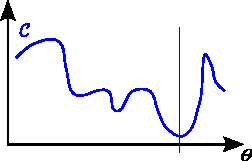
\includegraphics[width=0.5\textwidth]{cost_true.pdf}

%    \begin{minipage}{0.48\textwidth}
%        \textbf{\emph{Yes}}
%    \end{minipage}
%    \hfill
%    \begin{minipage}{0.48\textwidth}
%    %\emph{No}
%    \end{minipage}

%    %\vspace{1mm}

%    \begin{minipage}[t]{0.48\textwidth}
%        \vspace{0pt}
%    Learning minimizes a cost function $\color{blue}{\CC}$ with respect to
%    $\MM$ given a data distribution $p_D$

%    \end{minipage}
%    \hfill
%    \begin{minipage}[t]{0.48\textwidth}
%    %    \vspace{0pt}
%    %$\color{blue}{\CC}$ is \emph{not} available, but $\color{red}{\tilde{\CC}}$ based
%    %on the samples from $p_D$.

%    \end{minipage}

%\end{frame}

%\begin{frame}{Is Learning Optimization?}

%    \centering
%    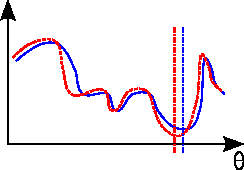
\includegraphics[width=0.5\textwidth]{cost_both.pdf}

%    \begin{minipage}{0.48\textwidth}
%        \textbf{\emph{Yes}}
%    \end{minipage}
%    \hfill
%    \begin{minipage}{0.48\textwidth}
%        \textbf{\emph{No}}
%    \end{minipage}

%    %\vspace{1mm}

%    \begin{minipage}[t]{0.48\textwidth}
%        \vspace{0pt}
%    Learning minimizes a cost function $\color{blue}{\CC}$ with respect to
%    $\MM$ given a data distribution $p_D$

%    \end{minipage}
%    \hfill
%    \begin{minipage}[t]{0.48\textwidth}
%        \vspace{0pt}
%    $\color{blue}{\CC}$ is \emph{not} available, but $\color{red}{\tilde{\CC}}$ based
%    on the samples from $p_D$.

%    \end{minipage}

%\end{frame}

\end{document}
